\documentclass[format=acmsmall, review=false, natbib=false]{acmart}
\usepackage{acm-ec-23}

\usepackage{biblatex} %Imports biblatex package
\addbibresource{ref.bib} %Import the bibliography file

\usepackage[ruled]{algorithm2e} % For algorithms
\renewcommand{\algorithmcfname}{ALGORITHM}
\SetAlFnt{\small}
\SetAlCapFnt{\small}
\SetAlCapNameFnt{\small}
\SetAlCapHSkip{0pt}
\IncMargin{-\parindent}

% Choose a citation style by commenting/uncommenting the appropriate line:

% submission mailbox: agtoffice2023@163.com
% email title: [Team#6] Project Milestone Report

\title{Project Milestone for Team$\#$6\\
	Double Auction Mechanism on Social Network
}
\author{Jintian Hu (2020533167), Huizhe Su (2020533009), Cheng Peng (2020533068), Liyu Yang (2020533162), Weiming Luo (2020533168)}

% Abstract. Note that this must come before \maketitle.

\begin{document}

% (1) Title, Authors, Student IDs
\maketitle

% (2) Brief Introduction: This section introduces your problem and the overall plan for approaching your problem.
\section{Introduction}
The overall plan for approaching the problem will involve conducting a literature review to establish connections between single seller mechanisms and our current multiple seller model, and using this information to develop a new mechanism that is suitable for our needs. After that, we will give some theoretical analysis on some key properties such as individual rationality (IR), incentive compatibility (IC), weak budget balance (WB), and economic efficiency (EE). If time permits, some simulation experiments will also be conducted as a supplement.




In recent years, research on double auctions has gained significant attention in the fields of economics and computer science. With the emergence of electronic markets, computer scientists are increasingly involved in the development of new market systems. Double auction markets can be viewed as centralized markets with specific trading rules where buyers and sellers conduct transactions according to regulations. A key issue in double auction research is to find a dominant strategy that allows sellers and buyers to genuinely report their respective valuations of merchandise.

In traditional double auction theory, we generally consider a fixed market consisting of buyers and sellers. However, in social networks, the absence of an effective double auction mechanism to facilitate the dissemination of information may lead to high valuation potential buyers missing out on auction information. Moreover, in traditional auctions, increasing profits for sellers and improving social welfare are usually two conflicting goals. By introducing the concept of social networking, we can motivate buyers who originally participated in the auction market to invite more potential buyers in the network to join, thus addressing both conflicting goals in traditional auctions simultaneously. It is crucial to design an auction mechanism that can achieve both advantages in social networks. However, the introduction of social networks means that we need to encourage buyers to not only report their merchandise valuations honestly but also disseminate auction information in social networks.

In this paper, we propose a novel scenario considering a social network with numerous interconnected sellers and buyers who conduct double auctions and incentivize buyers to invite neighbors to participate in the auction. Unlike existing research, our scenario focuses on intersecting buyer groups and the interconnections between buyers. This implies that a buyer may belong to multiple buyer groups simultaneously. Our goal is to find a double auction mechanism that motivates all buyers to invite other potential buyers in the social network while maintaining the advantages of traditional mechanisms, which cannot be achieved under existing mechanisms.

To address this issue, we first design a new double auction model in which buyers can interact with their neighbors in the social network and share auction information. In this model, we specifically focus on intersecting buyer groups and the mutual connections between buyers. Next, we propose and analyze a new auction mechanism that possesses incentive compatibility (IC) in the social network, meaning that honestly reporting true valuations is the optimal strategy for participants. We also study the performance of this mechanism in handling intersecting buyer groups, including aspects such as social welfare and budget balance.

To validate the effectiveness of our proposed auction mechanism, we prove its incentive compatibility through theoretical analysis. In addition, we conduct a series of simulation experiments to evaluate the performance of the mechanism under various conditions. The experimental results show that our auction mechanism achieves relatively high social welfare while maintaining budget balance when dealing with intersecting buyer groups, thereby addressing the two conflicting goals in traditional auctions to a certain extent.


% (3) Clear Model: Describe your problem precisely specifying the setting and assumptions.
\section{The Model}
Consider a double auction market of $n+m$ participants
where $n$ out of them are sellers and the rest $m$ participants are potential buyers. Let $S=\{s_1,s_2,\ldots, s_n\}$ and $B=\{b_1,b_2,\ldots b_m\}$ be the set of all sellers and buyers.
Each seller $s_i\in S$ is holding a one-unit item and is willing to sell it at price no lower than $v^s_i$. Each buyer $b_j\in B$ wants to purchase one item with price no more than $v^b_j$.

Every participant of the market is connected to some other participants forming a social network. More precisely, every seller or buyer $x\in S\cup B$ can only communicate directly with its neighbors $r_x\subseteq (S\cup B\setminus \{x\})$.
Initially, only part of the buyers (called head buyers) are aware of the incoming auction.
Head buyers are those who is directly linked to a seller.
$H = \bigcup_{s_i \in S} (r_x \cap B)$ denotes all the head buyers in the market.


To sell the item at higher price, the sellers want to invite potential buyers other than the initial ones i.e, the head buyers, to expand the auction.
However, once neighboring potential buyers are invited to the auction, they will compete with the initial buyers for the items. Intuitively, a buyer has incentive to keep his neighboring buyers from entering the market.
Therefore, the market owner must adopt a mechanism encouraging the buyers in the market to inform the neighbors not being aware of the auction.

A mechanism for double auction on social network requires the buyers and the sellers to report their private information and decide the allocation of items and payment for each agent.
For the sellers, the mechanism asks them to reveal their expected price $\hat v^s=(\hat v^s_1,\hat v^s_2,\ldots \hat v^s_n)$.
The mechanism also requires the buyers to report their type $\hat\theta_i = (\hat v^b_i, \hat r_{s_i})$ and use $\hat\theta = (\hat\theta_1,\hat\theta_2,\ldots,\hat\theta_m)$ to denote a reported type profile.

After receiving the reported information $\hat\theta$ and $\hat v^s$, the mechanism determines the allocation $\pi^s,\pi^b$ and the payment $p^s,p^b$.
\begin{itemize}
	\item For each seller $s_i$:
		The allocation $\pi^s_i = 1$ means that he can trade the item with a buyer, otherwise $\pi^s_i = 0$.
		The payment $p^s_i\leq 0$ gives the money $s_i$ can get from the market owner.
	\item For each buyer $b_i$:
		The allocation $\pi^b_i = 1$ indicates that he get one item from a seller while $\pi^b_i=0$ if he get no item.
		The payment $p^b_i>0$ if $b_i$ is asked to pay money to the market owner
		and $p^b_i<0$ when $b_i$ can get get some rewards from the market owner.
\end{itemize}


We make a few definition of properties for further discussion.

\begin{definition}[active buyers]
	Given a profile $\hat\theta$, we say buyer $b_i$ is active
	if there exists $q_1,q_2,\ldots q_k in [1,n]$ such that
	$b_{q_1}\in H$ is a head buyer, $b_{q_k}=b_i$ is the active buyer and
	$b_{q_{i+1}} \in \hat r_{b_{q_i}}$ for every $i=1,2\ldots k-1$.
	That is a buyer is active if he is a head buyer or an active buyer invites him.\\
	Let $Q\subseteq B$ be the set of all active buyers.
\end{definition}

Next we definition the desired properties of the mechanism.

\begin{definition}[valid]
	A mechanism is valid if for all possible input of $(\hat\theta,\hat v^s)$ the following conditions are satisfied.
	\begin{itemize}
		\item If $b_i\not\in Q$ then $\pi^b_i=p^b_i=0$.
		\item $\sum_{b_i\in B} \pi^b_i = \sum_{s_i\in S} \pi^s$.
	\end{itemize}
\end{definition} 

\begin{definition}[utility]
	The utility is the welfare an agent gains from participanting the double auction mechanism trading.
	\begin{itemize}
		\item For $b_i\in B$, his utility is $u^b_i = \pi^b_i v^b_i-p^b_i$.
		\item For $s_i\in S$, his utility is $u^s_i = \pi^s_i v^s_i-p^s_i$.
	\end{itemize}
\end{definition}

\begin{definition}[individual rational (IR)]
	A mechanism is IR if for all possible input of $(\hat\theta,\hat v^s)$,
	\begin{itemize}
		\item For all $b_i\in B$, $u^b_i((\theta_i,\hat\theta_{-i}),\hat v^s)\geq 0$.
		\item For all $s_i\in S$, $u^s_i(\hat\theta,(v^s_i, \hat v^s_{-i})\geq 0$.
	\end{itemize}
	That is, no agent is punished for participating truthfully.
\end{definition}

\begin{definition}[incentive compatible (IC)]
	A mechanism is IC if
	\begin{itemize}
		\item For all $b_i\in B$,
			$u^b_i((\theta_i,\hat\theta_{-i}),\hat v^s)
			\geq u^b_i(\hat\theta,\hat v^s)$.
		\item For all $s_i\in S$,
			$u^s_i(\hat\theta,(v^s_i,\hat v^s_{-i}))
			\geq 
			u^s_i(\hat\theta,\hat v^s)$
	\end{itemize}
	That is, an agent's utility is maximized when he participate truthfully.
\end{definition}

\begin{definition}[weak budget balance (WBB)]
	A mechanism is WBB if
	$\sum_{s_i\in S} p^s_i(\hat\theta,\hat v^s)
	+\sum_{b_i\in B} p^b_i(\hat\theta,\hat v^s) \geq 0$
	for all $(\hat\theta,\hat v^s)$.
	That is, the market owner never pay extra money for running the mechanism.
\end{definition}


% (4) Technical Approach: Describe the methods you intend to apply to solve the given problem Intermediate/Preliminary.
\section{Technical Approach}
Given the current model and prior works, we would like to design a novel double auction mechanism
on social network that satisfies Individual Rational(IR), Incentive Compatible(IC) and Budget Balance(BB).
However, by Myerson-Satterthwaite theorem[need cite], it's impossible to also guranteen the
Economic Efficiency. Therefore, our mechanism will be slightly inefficient since it will not
guranteen that the buyer with higher elvaluation will always get the item.\par
After that, we will give an exhaustive analysis of our mechanism, with thorogh proofs on
IR, IC, and BB. For EE, we will try to give a bound analysis, to see how worse the social warefare
can be compared to the most efficient one. If time permits, we will also carry out a simulation
of our mechanim.


% (5) Results: State and evaluate your results up to the milestone.
\section{Current Results}
We have made several attempts to adapt existing mechanisms into our model.
\subsection{DNA on Connected Network}
One of the outstanding works on double auctions on social networks is Double Network Auction (DNA)\cite{DNA}. The method is an extension of McAfee's trade reduction mechanism
that runs on several disjoint buyer networks. Therefore, we may reduce our model to DNA's model
by dividing the connected buyer networks into several disjoint smaller buyer networks according to the allocation
given by McAfee's method.
However, we can find a situation where the network is individable. Fig \ref*{fig:DNACounter}
shows one of the situations when several sellers together are connected to a chain of buyers. Therefore,
our problem setting cannot be reduced.
\begin{figure}[htbp]
  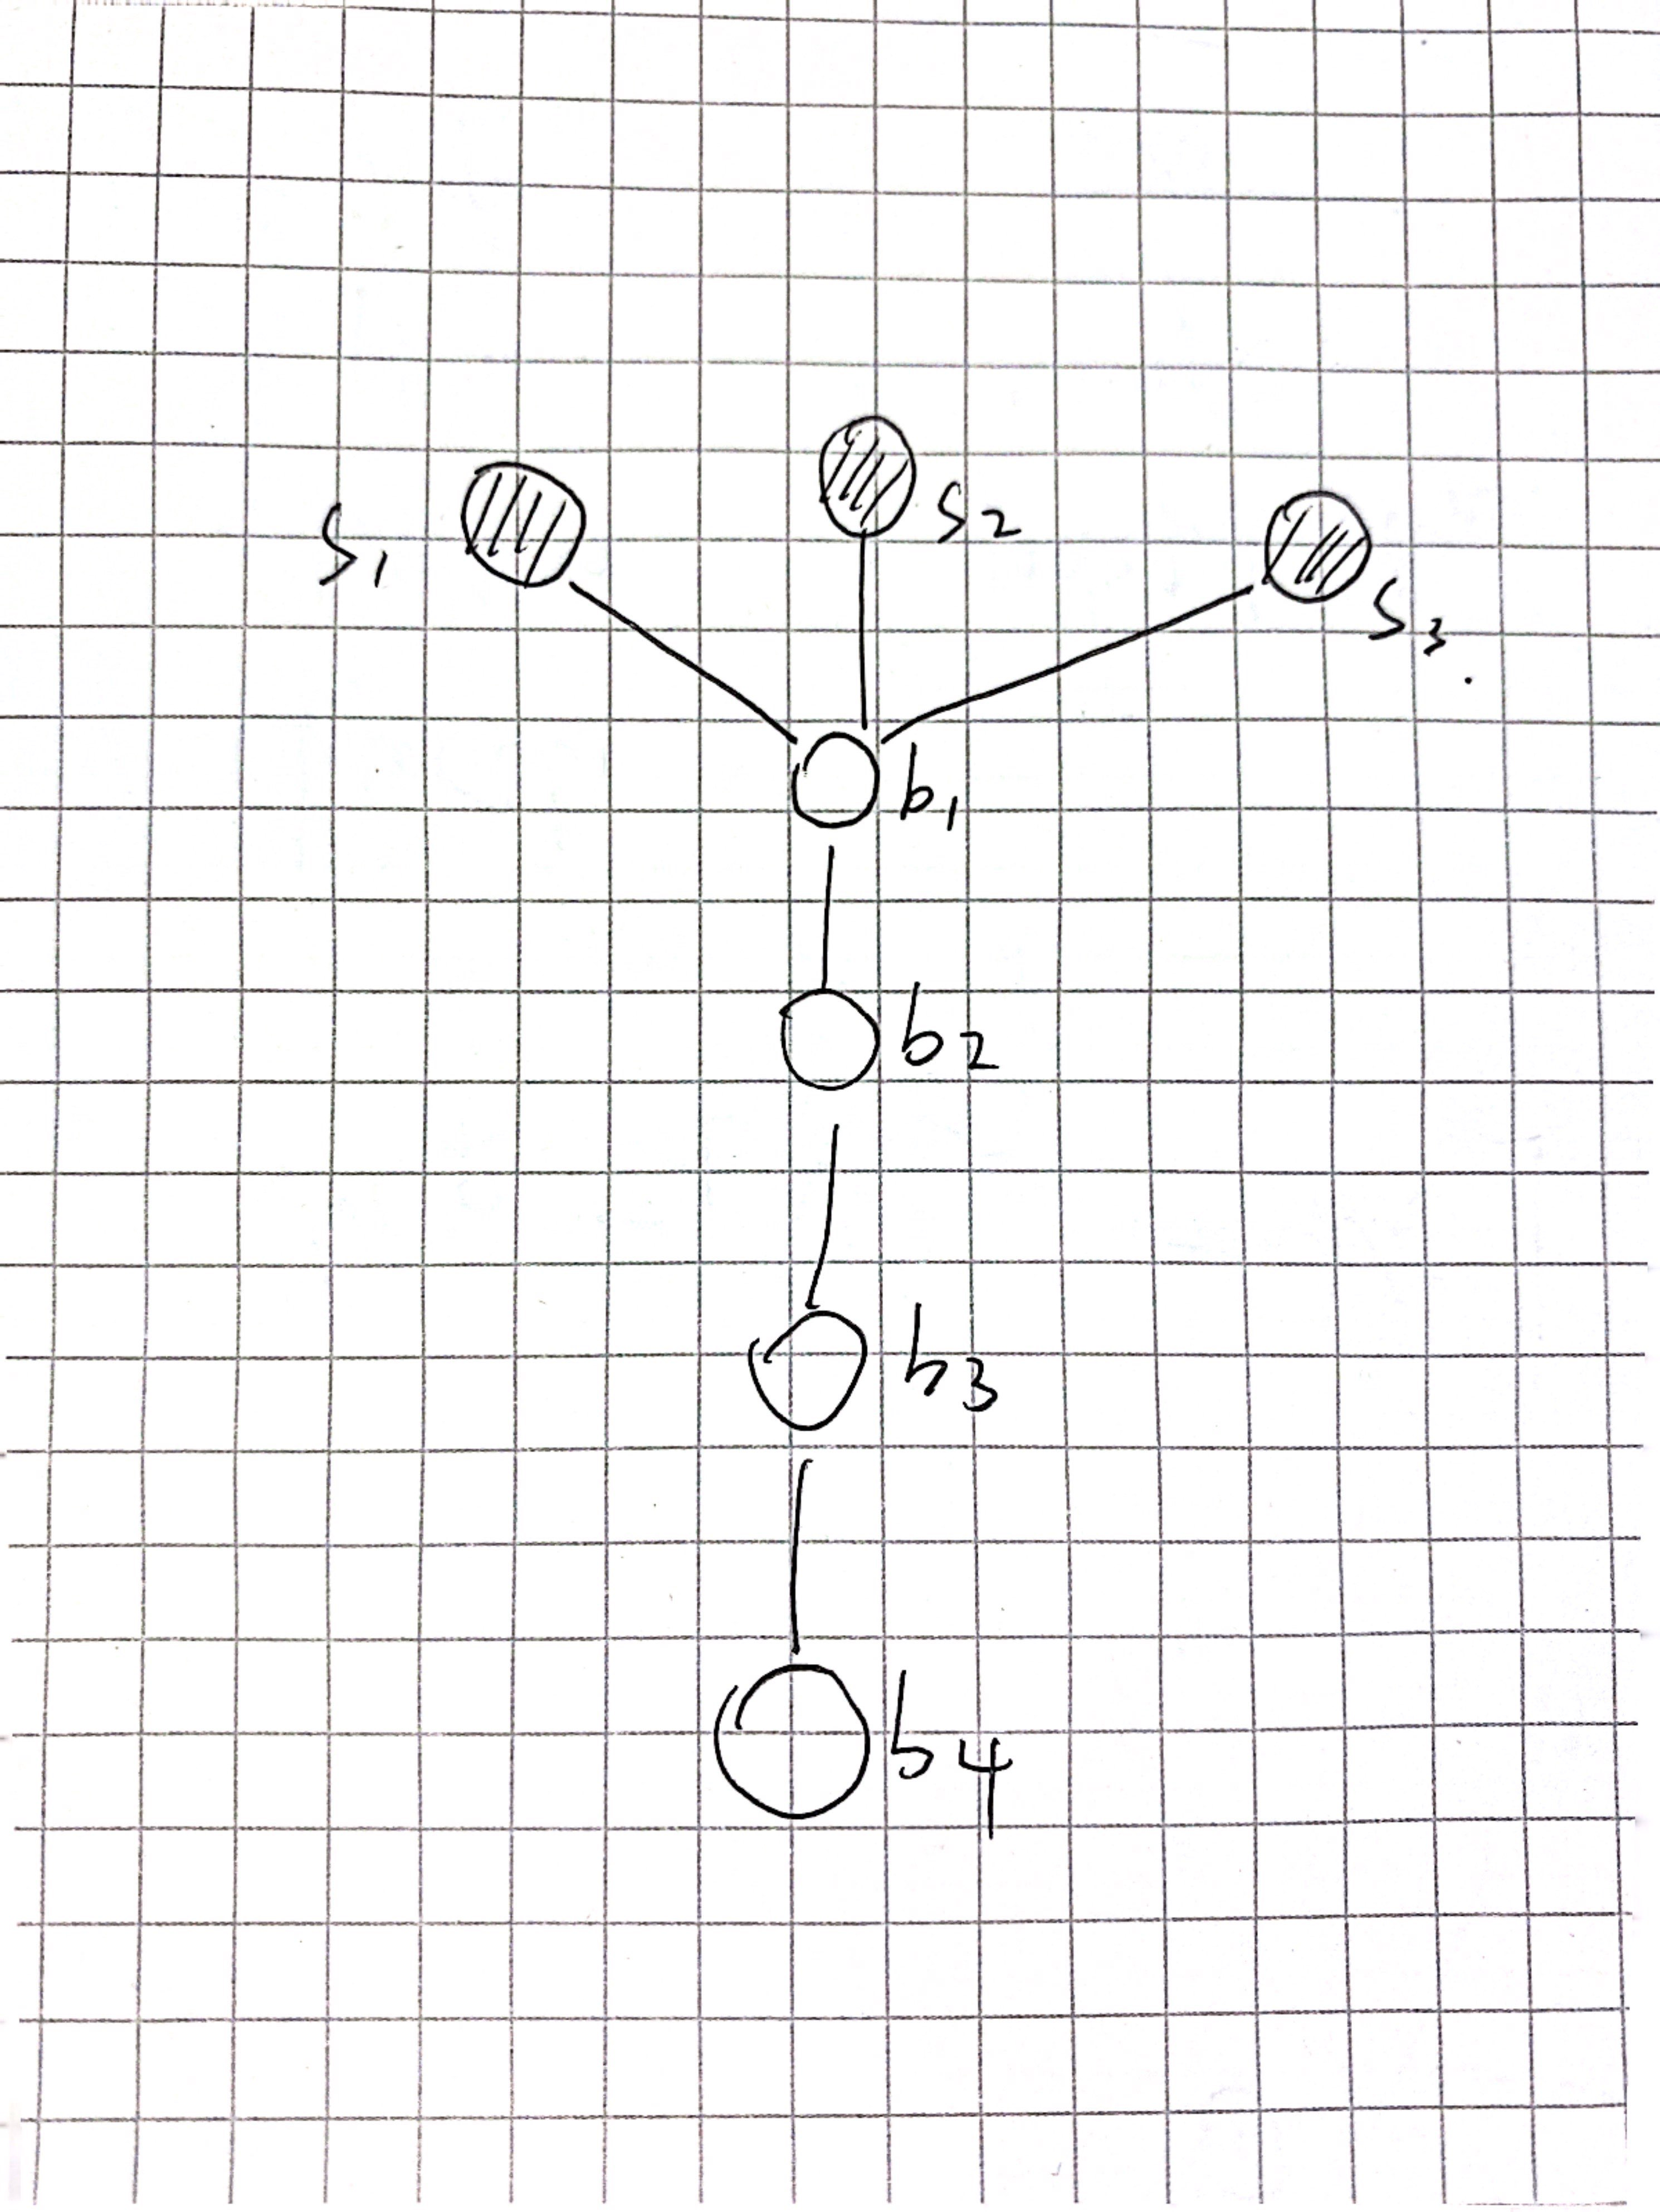
\includegraphics[width=0.6\textwidth]{./figure/DNA_counter_1.jpg}
  \caption{Network that can not be divided}
  \label{fig:DNACounter}
\end{figure}
\subsection{Multi-item Mechanism}
In a double auction scenario, we have multiple sellers, which means we also have multiple items. Therefore,
the multi-item mechanism may provide some valuable insights.\par
First, we try to adapt Generalized IDM(GIDM)\cite{GIDM} and Distance-based Network Auction mechanism for Multi-unit, Unit-demand buyers(DNA-MU)\cite{DNA-MU}.
However, these two methods are not IC. The counterexample is given in \ref*{fig:GIDMCounter}. The seller has
\(m = 4\) items. The example is from \cite{MUDAN-MUDAR}.
\begin{figure}[htbp]
  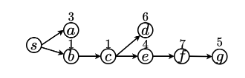
\includegraphics{./figure/GIDM_counter.png}
  \caption{Counter example for both GIDM and DNA-MU}
  \label{fig:GIDMCounter}
\end{figure}
\begin{itemize}
  \item \textbf{GIDM} If all player report truthfully. The winner will be \(b,c,d,e\)(Table \ref*{table:GIDMTruthful}).
        However, if \(f\) misreport her connection, then the allocation result will be \(a,b,c,f\)
        (Table \ref*{table:GIDMMisreport}).
        \begin{table}[htbp]
          \begin{tabular}{c|c|c|c}
            round & left items & winners         & \(\pi, p\)             \\
            \hline
            1     & 4          & \(\varnothing\) & \(\pi_b = 1, p_b = 0\) \\
            2     & 3          & \(\{b\}\)       & \(\pi_c = 1, p_c = 0\) \\
            3     & 2          & \(\{b,c\}\)     & \(\pi_d = 1, p_d = 5\) \\
            4     & 1          & \(\{b,c,d\}\)   & \(\pi_e = 1, p_e = 3\) \\
            \hline
          \end{tabular}
          \caption{GIDM with \(m = 4\). All buyer report truthfully\cite{MUDAN-MUDAR}}
          \label{table:GIDMTruthful}
        \end{table}
        \begin{table}[htbp]
          \begin{tabular}{c|c|c|c}
            round & left items & winners         & \(\pi, p\)             \\
            \hline
            1     & 4          & \(\varnothing\) & \(\pi_a = 1, p_b = 0\) \\
            2     & 3          & \(\{a\}\)       & \(\pi_b = 1, p_c = 0\) \\
            3     & 2          & \(\{a,b\}\)     & \(\pi_c = 1, p_d = 0\) \\
            4     & 1          & \(\{a,b,c\}\)   & \(\pi_f = 1, p_e = 6\) \\
            \hline
          \end{tabular}
          \caption{GIDM with \(m = 4\). \(f\) misreport connection \(r'_f = \varnothing\)\cite{MUDAN-MUDAR}}
          \label{table:GIDMMisreport}.
        \end{table}
  \item \textbf{DAN-MU} If all player report truthfully. The winner will be \(b,c,d,e\)
        (Table \ref*{table:DAN-MUTruthful}).
        However, if \(f\) misreport her connection, then the allocation result will be \(a,b,c,f\)(Table \ref*{table:DAM-MUMisreport}).
        \begin{table}[htbp]
          \begin{tabular}{c|c|c|c}
            round & left items & agent & \(\pi, p\)             \\
            \hline
            1     & 4          & \(b\) & \(\pi_b = 1, p_b = 0\) \\
            2     & 3          & \(c\) & \(\pi_c = 1, p_c = 0\) \\
            3     & 2          & \(d\) & \(\pi_d = 1, p_d = 5\) \\
            4     & 1          & \(e\) & \(\pi_e = 1, p_e = 3\) \\
            \hline
          \end{tabular}
          \caption{DAN-MU with \(m = 4\). All buyer report truthfully\cite{MUDAN-MUDAR}}
          \label{table:DAN-MUTruthful}
        \end{table}
        \begin{table}[htbp]
          \begin{tabular}{c|c|c|c}
            round & left items & agent & \(\pi, p\)             \\
            \hline
            1     & 4          & \(a\) & \(\pi_a = 1, p_b = 1\) \\
            2     & 3          & \(b\) & \(\pi_b = 1, p_c = 0\) \\
            3     & 2          & \(c\) & \(\pi_c = 1, p_d = 0\) \\
            4     & 1          & \(f\) & \(\pi_f = 1, p_e = 6\) \\
            \hline
          \end{tabular}
          \caption{DAN-MU with \(m = 4\). \(f\) misreport connection \(r'_f = \varnothing\)\cite{MUDAN-MUDAR}}
          \label{table:DAN-MUMisreport}.
        \end{table}
\end{itemize}
We can reduce our
problem to a multi-item problem if we connect several sellers to the same buyer with the same prices.
An example is shown in Fig \ref*{fig:MultiReduce}. It can be expected that the adapted method will not be IC either.\par
\begin{figure}[htbp]
  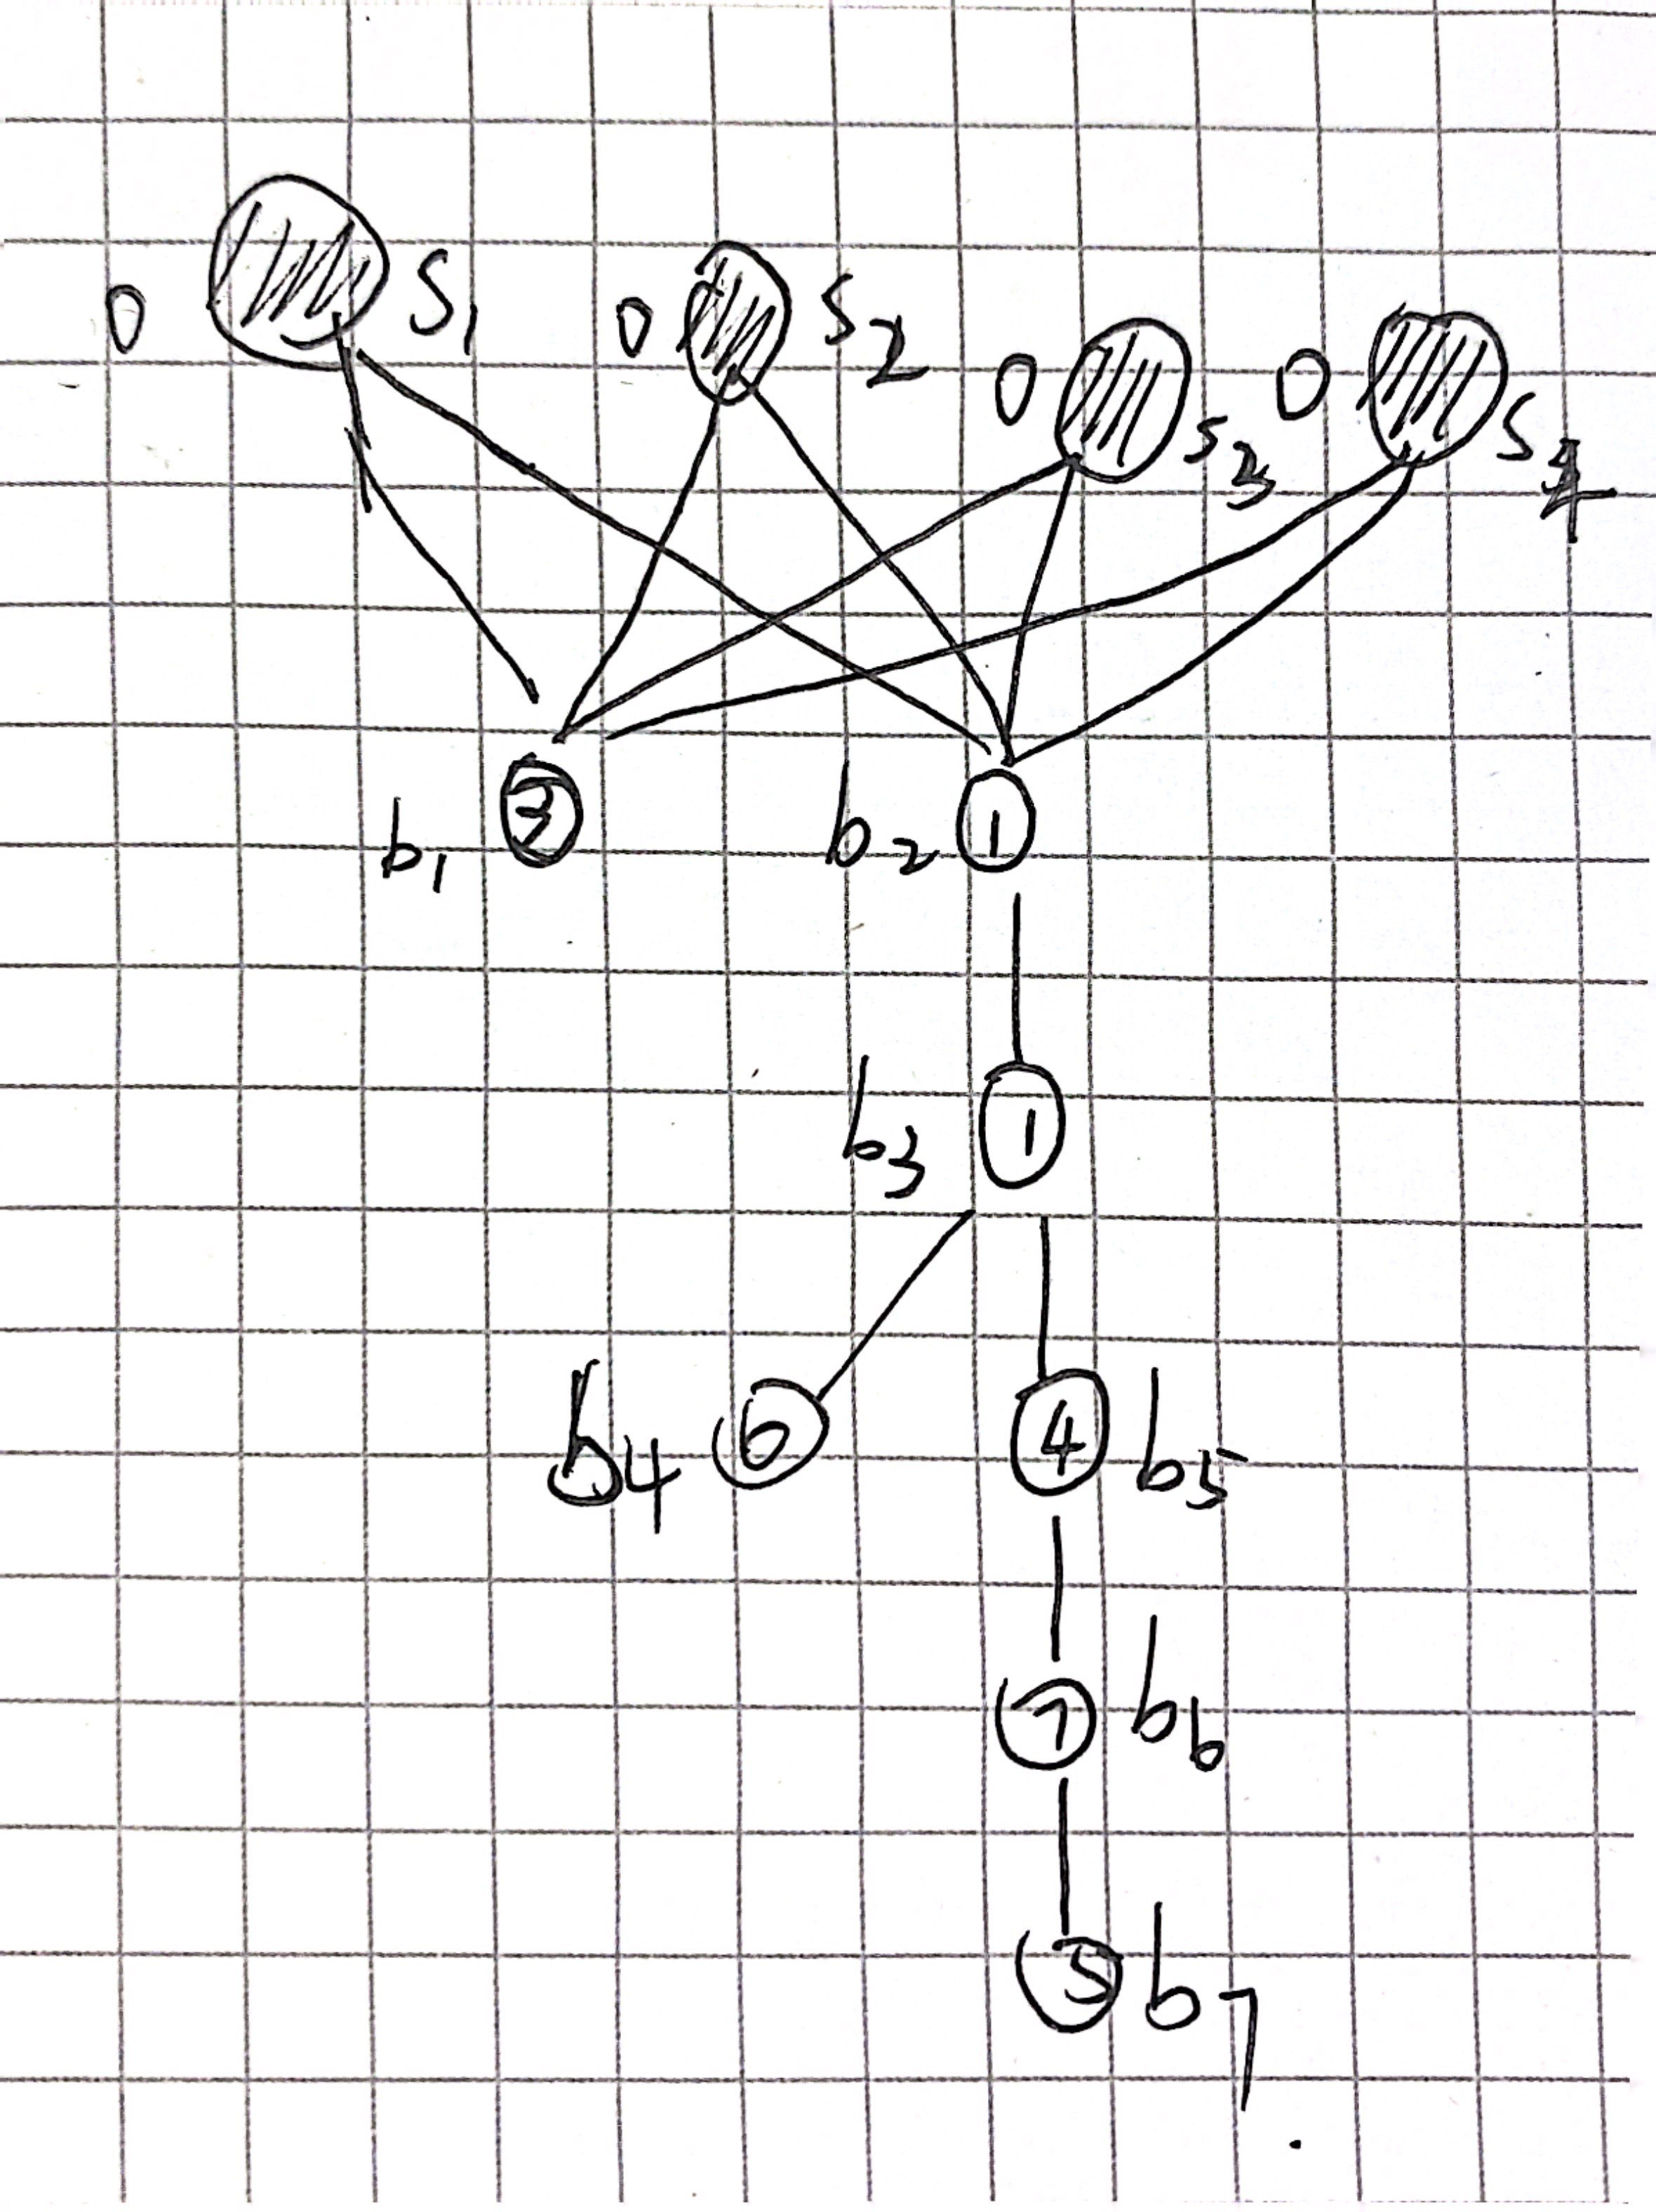
\includegraphics[width=0.6\textwidth]{figure/Multi_reduce.jpg}
  \caption{A reduction from multi-seller to multi-item}
  \label{fig:MultiReduce}

\end{figure}

We also look into two other IC mechanisms: MUDAN and LDM. These two methods are both layer-based mechanisms.
In our setting, items are held by different sellers. If the sellers are scattered around the network, the
network will degenerate into one layer since the children cannot get them, even if they may have higher
evaluations. An example is shown in Fig \ref*{fig:LayerDegenerate}.
\begin{figure}
  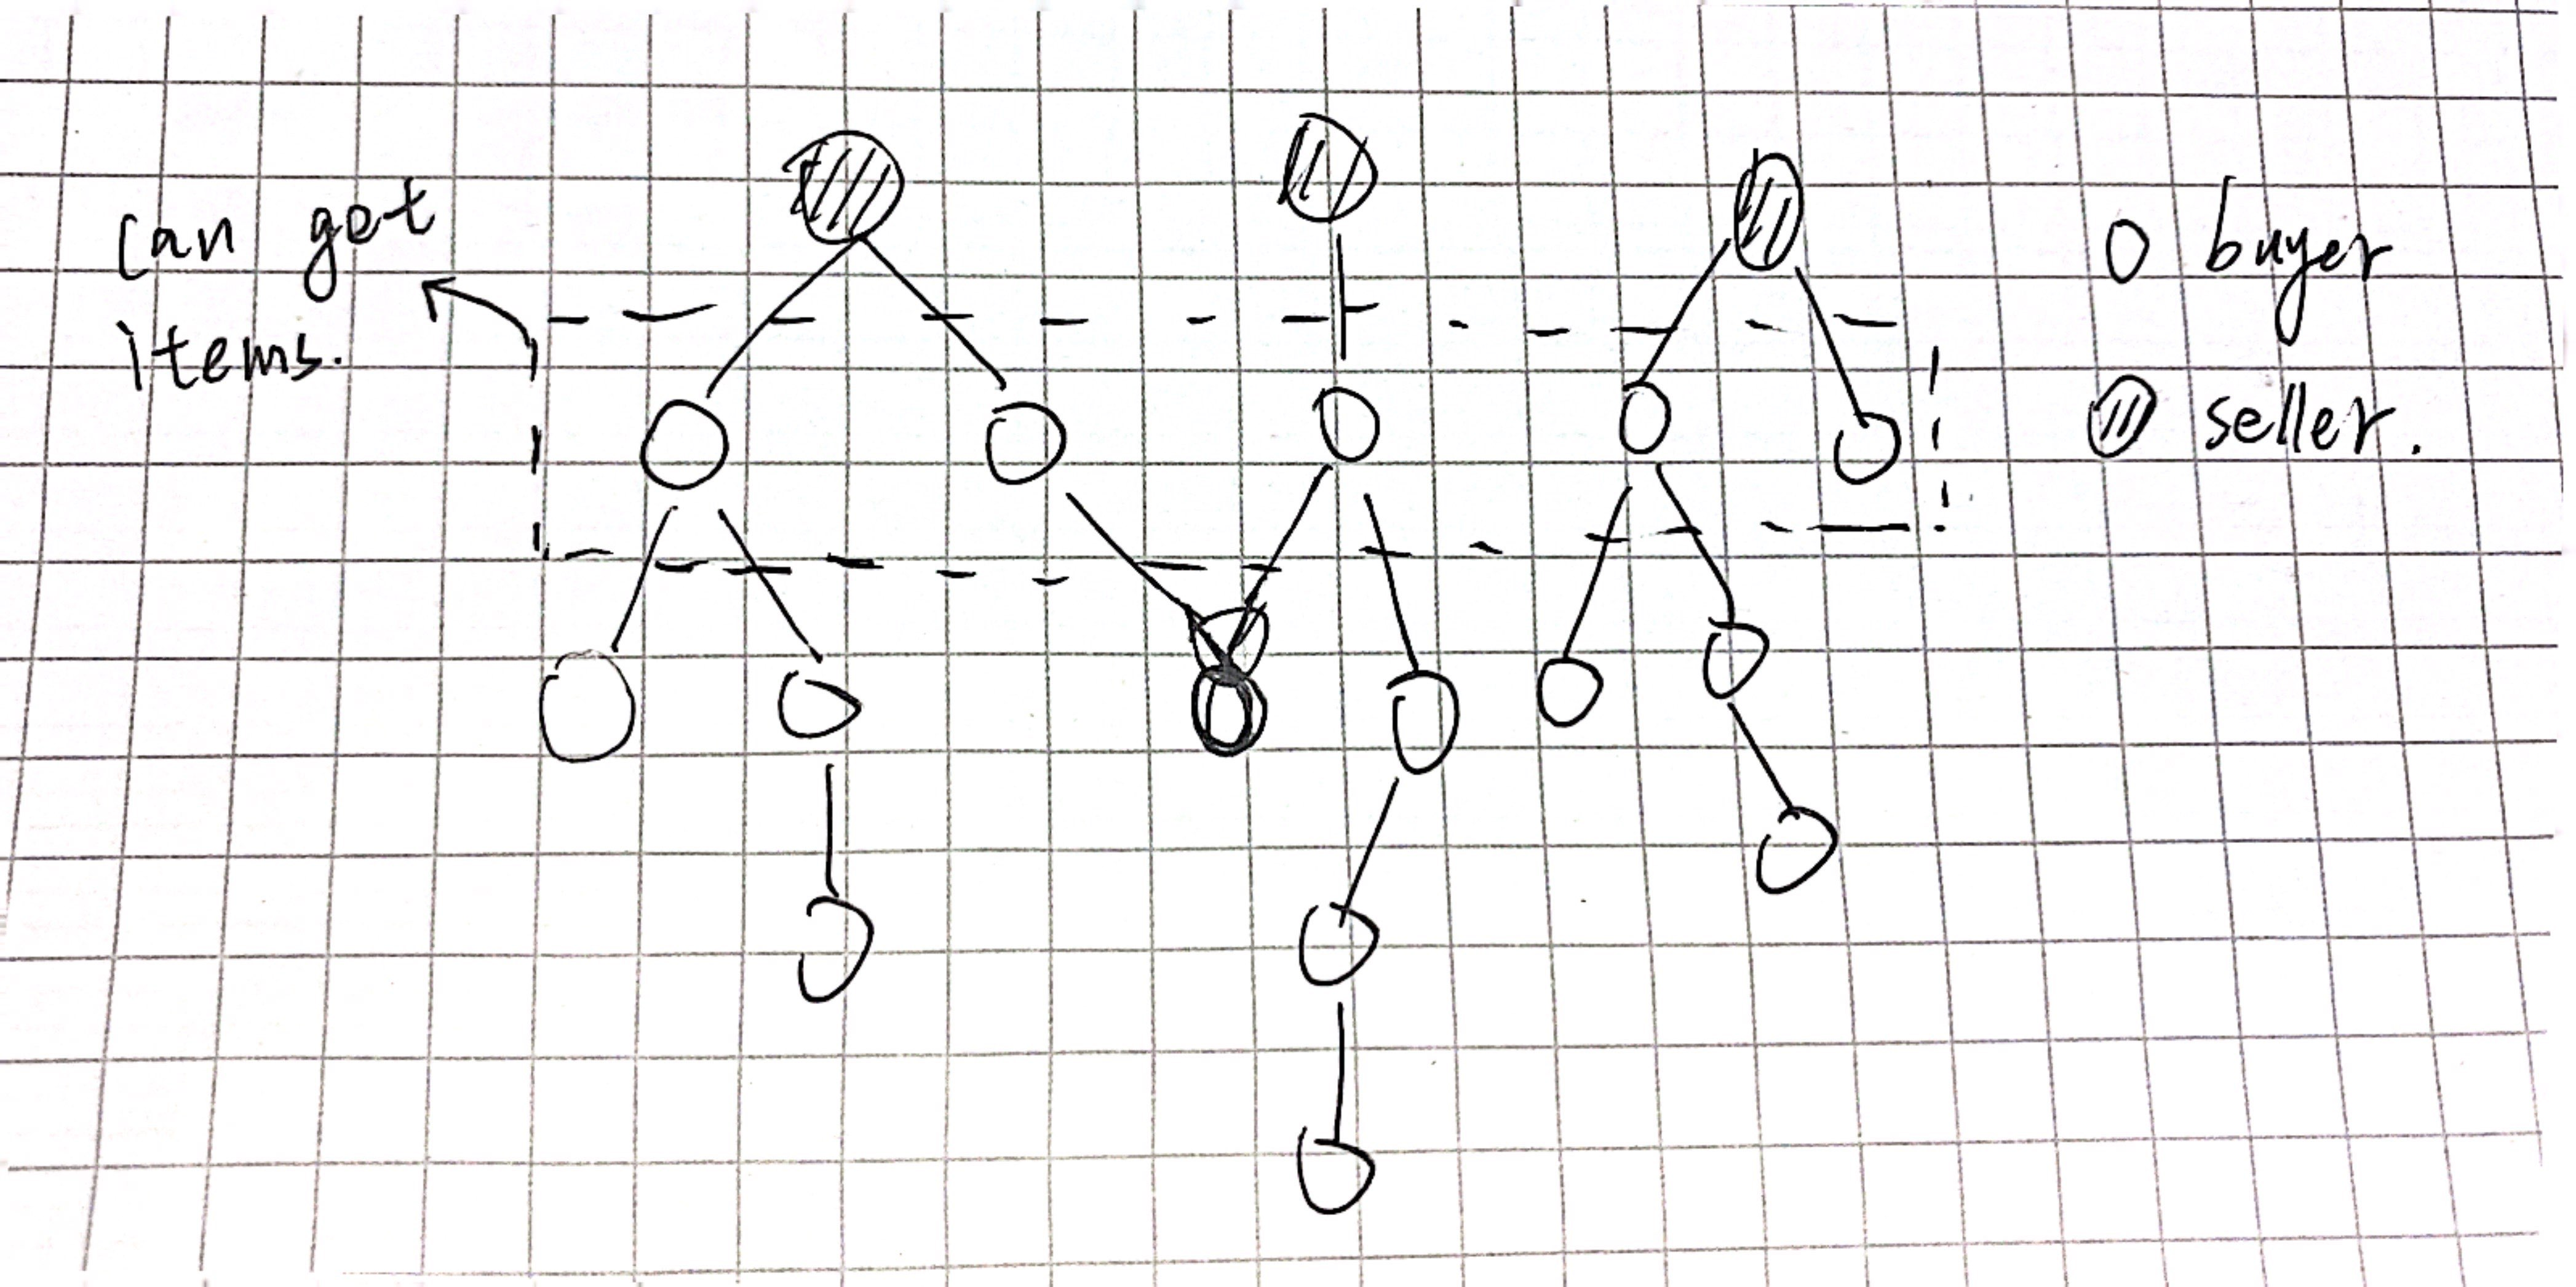
\includegraphics[width=0.6\textwidth]{./figure/Layer_degenerate.jpg}
  \caption{An example of the degeneration of a network to a single layer. }
  \label{fig:LayerDegenerate}
\end{figure}
\subsection*{Resale mechanism with leave and share}
In double-auction, we want people with high valuations to hold the item. Therefore, resale mechanisms are better than
layer-based mechanisms. Buyers with higher evaluations have more chances to get the item, while buyers with lower
evaluations are rewarded if they invite someone who gets it. From this insight, we designed a naive
resale mechanism that combined IDM with leave and share. The mechanism is described as follows,
\begin{enumerate}
  \item Sort the sellers in order of their price from lowest to highest.
  \item Let the seller with the lowest price sell the item using IDM. Other sellers are viewed as buyers with 0 valuations.
  \item The seller and the winner leave the network and share their connection.
  \item Repeat step 2, 3 until no seller can sell the item.
\end{enumerate}
However, this mechanism is not IC since the seller with a lower price has more chance to sell their
item at a high price, and the seller has the incentive to misreport a lower price. In the following example, if \(s_1\)
\(s_2\) both report truthfully (Fig \ref*{fig:LeaveTruthful}), then \(s_2\) will receive \(9\). But
if he misreport \(2\), he will receive \(10\)(Fig \ref*{fig:LeaveMisreport}). Therefore, he has the incentive to misreport.
\begin{figure}[htbp]
  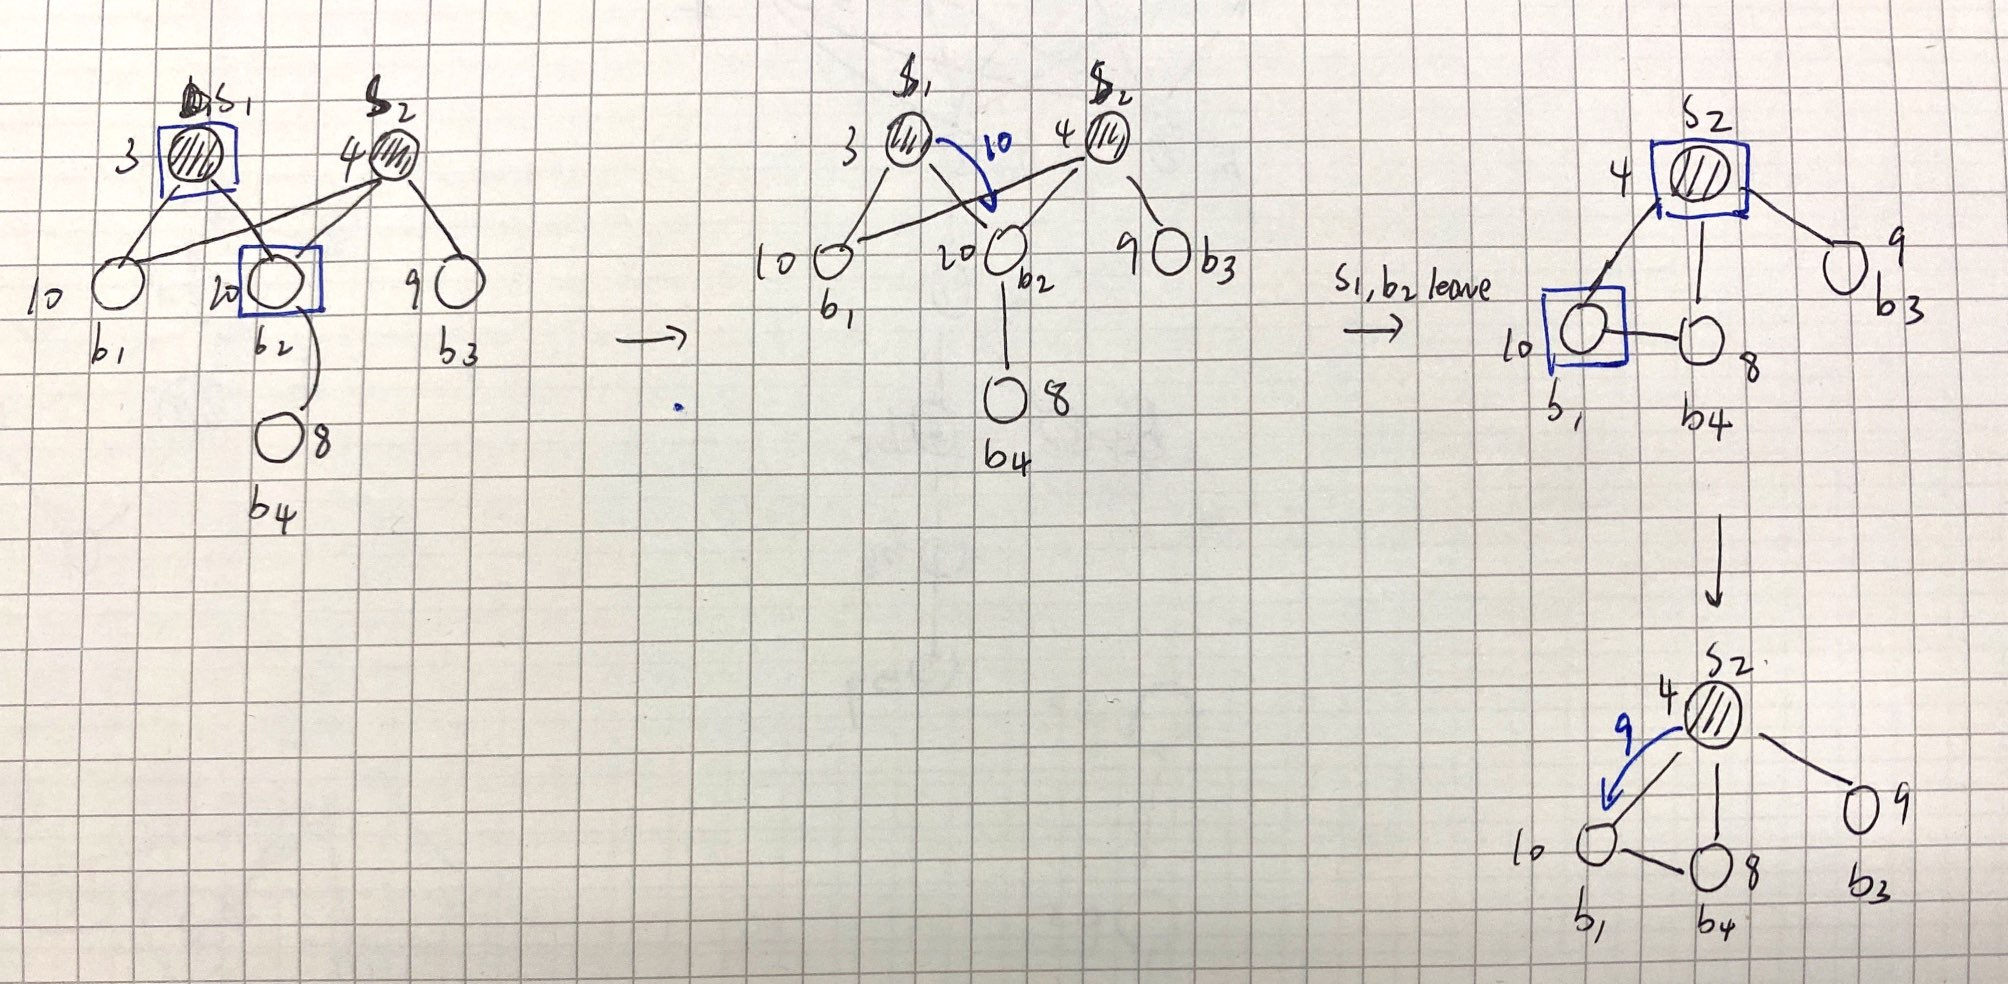
\includegraphics[width=0.6\textwidth]{figure/Leave_truthful.jpg}
  \caption{A run of the naive algorithm. All player report truthfully}
  \label{fig:LeaveTruthful}
\end{figure}
\begin{figure}[htbp]
  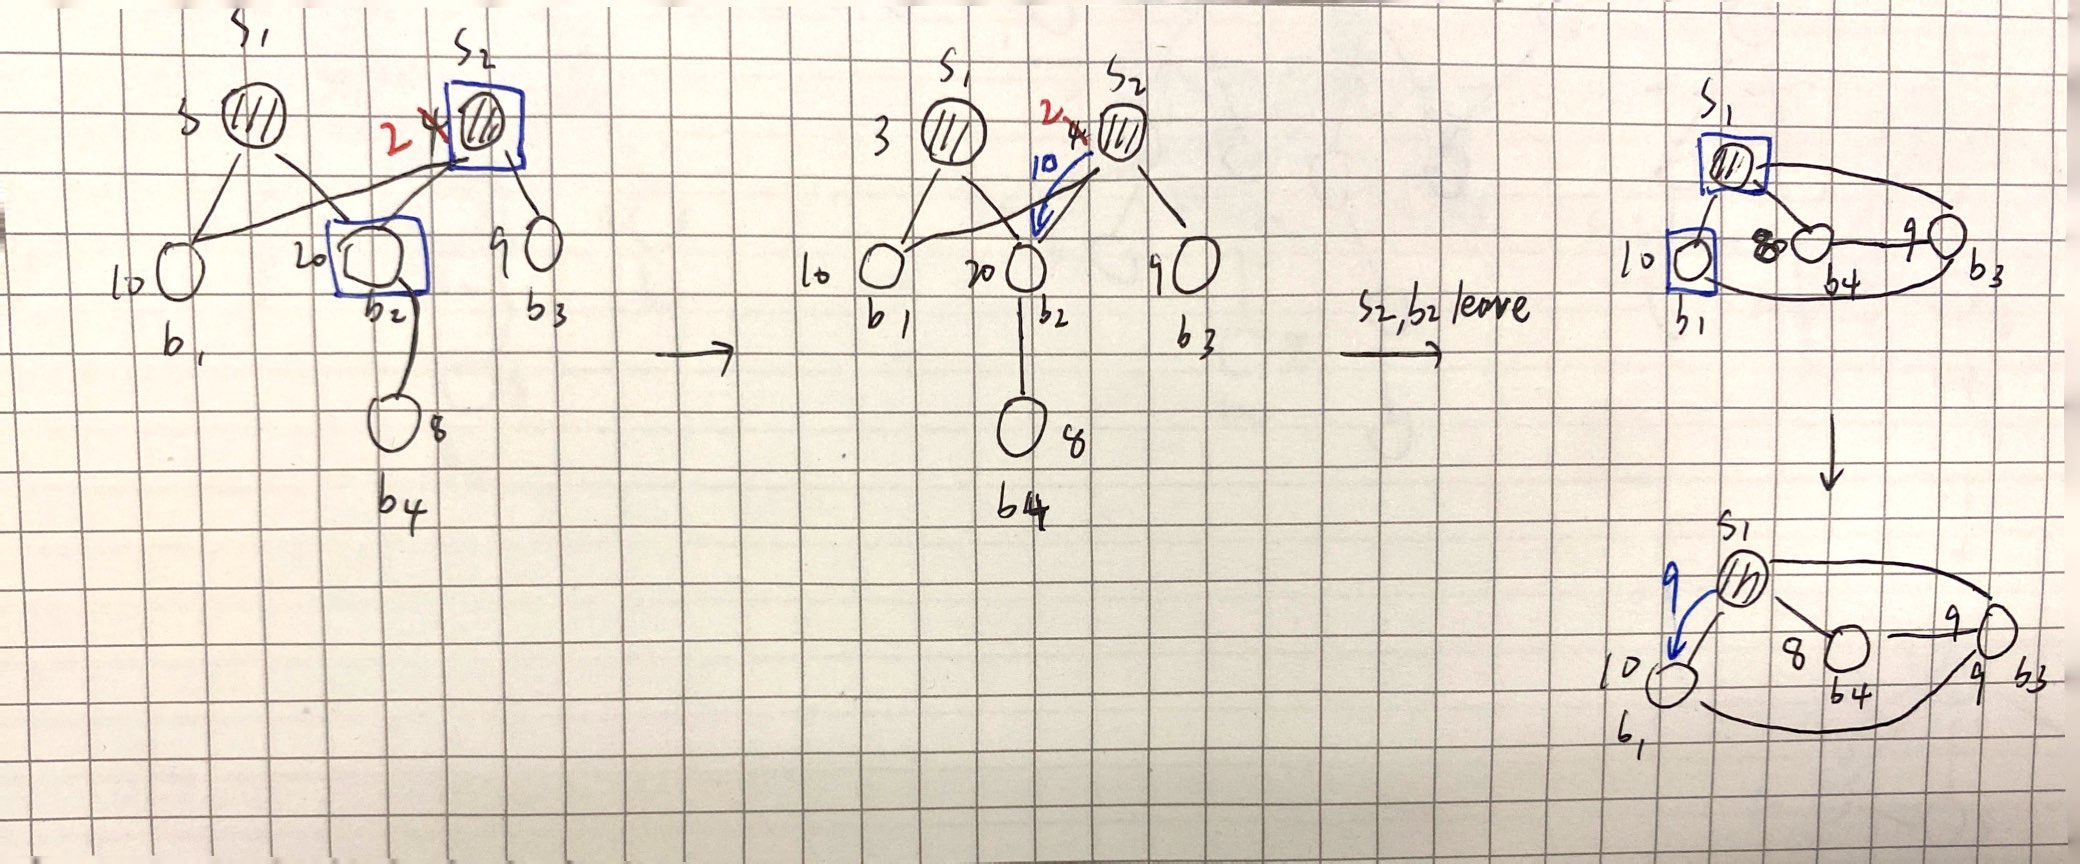
\includegraphics[width=0.6\textwidth]{figure/Leave_misreport.jpg}
  \caption{A run of the naive algorithm. \(s_2\) misreport \(2\)}
  \label{fig:LeaveMisreport}
\end{figure}

\subsection*{Resale with leave and share, eliminating highest \(m\) bid}
Then we modified the original algorithm. The main idea is still the same, but when calculating
the price using IDM, we first eliminate the highest \(m\) bids, where \(m\) is the number of unmatched sellers.
As a result, the seller cannot profit more by misreporting, and neither can the buyer. However, we still have to do
more work to show and prove that this mechanism is IC.
Moreover, Since we have eliminated the highest bids, some deals that might have worked will fail.
However, this will not be a problem if the network is big enough and the number of the buyer is much greater than the seller.

\nocite{*}
\printbibliography
\end{document}
